\begin{frame}
\frametitle{The Parable of the listreverse project}
\begin{center}
Imagine, for a minute, a programming language that did not allow the programmer to generalise on list element types \ldots
\end{center}
\end{frame}

\begin{frame}
\frametitle{The Parable of the listreverse project}
\begin{center}
\ldots and if you wanted to reverse a list of bananas, you would solve that problem specific to bananas. 
\end{center}
\end{frame}

\begin{frame}[fragile]
\frametitle{The Parable of the listreverse project}
\begin{itemize}
\item<1-> But what if we then had to also reverse a list of oranges?
\item<2-> Well, we would copy and paste the previous code :)
\end{itemize}
\end{frame}

\begin{frame}
\frametitle{The Parable of the listreverse project}
Soon enough, there would be a listreverse project and contributors, with all the different list reversals.
\vfill
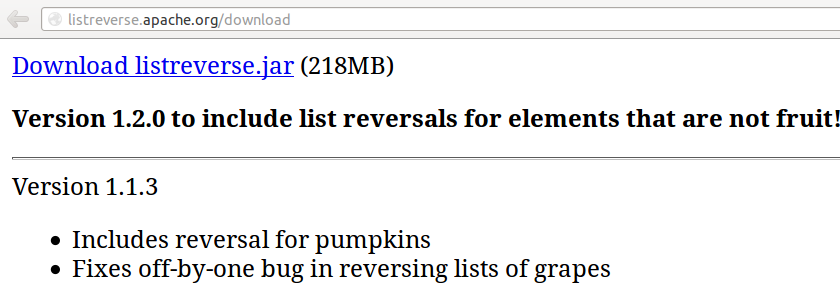
\includegraphics[height=0.3\textheight,natwidth=840,natheight=285]{image/listreverse.png}
\end{frame}

\begin{frame}
\frametitle{The Parable of the listreverse project}
\begin{block}{So, you asked\ldots}
Why don't we use a programming environment that supports reversal on \emph{any} element type?
\end{block}
\end{frame}

\begin{frame}
\frametitle{The Parable of the listreverse project}
\begin{block}{and you were told\ldots}
\begin{quote}
The listreverse project is doing just fine and is used in many enterprise projects and has many contributors successfully incorporating it into their solutions.
\end{quote}
\end{block}
\end{frame}

\begin{frame}
\frametitle{The Parable of the listreverse project}
\begin{block}{The reason}
These interfaces are not exploited is due to \emph{unfamiliarity} and tool support that discourages exploitation providing the perception of progress.
\end{block}
\end{frame}
